\section{Formalisations théoriques}\label{sec:rw:sgfd:modeles}
Nous avons présenté brièvement dans le chapitre~\ref{chap:rw:supervision} que les systèmes de gestion de flux de données s'inspiraient du modèle relationnel. Le modèle relationnel ne permet toutefois pas l'interrogation de données en temps réel. Ainsi, de nombreuses propositions ont été faites pour construire un modèle intégrant les flux tout en tentant de réutiliser les connaissances développées sur les systèmes de gestion de base de données relationnels depuis 40 ans.

Dans cette section, nous détaillons l'historique de la recherche dans le domaine de la gestion de flux. Observer l'évolution des modèles au fur et à mesure des années permet en effet de cerner les problématiques théoriques liées à la gestion de flux. En~\ref{sec:rw:sgfd:modeles:early}, nous présentons les premiers modèles. En~\ref{sec:rw:sgfd:modeles:stream}, nous présentons la sémantique abstraite mélangeant flux et relations. Puis, nous présentons en~\ref{sec:rw:sgfd:modeles:batch} les initiatives de clarification et reformalisation des modèles existants.

\subsection{La genèse de la gestion de flux}\label{sec:rw:sgfd:modeles:early}
L'idée de créer des requêtes continues a été présentée en 1992 dans le système Tapestry~\cite{Terry:tapestry}. Dans ce système une requête continue est avant tout une requête instantanée exécutée périodiquement. Ces requêtes s'appliquent sur un ensemble de données sans suppression ou mise à jour (\textit{append-only}). Le résultat est représenté par le flux des nouvelles données calculées de manière incrémentale. Pour cela, les relations sont considérées comme des variables et elles deviennent dépendantes du temps.

En 1995, les flux de données ont été explorés tout d'abord par le modèle séquentiel $\mathcal{SEQ}$~\cite{Seshadri:seq}. Dans ce modèle, une \enquote{\it séquence} est un ensemble d'enregistrements (n-uplets relationnels) avec un ordre positionnel. Dans le modèle relationnel originel~\cite{Codd:model}, ceci n'est pas autorisé, car l'ordre des n-uplets est dit \enquote{\it irrelevant}. La sémantique de spécification des opérateurs relationnels utilise cette liberté d'ordre pour être consistante et obtenir des propriétés intéressantes (voir chapitre~\ref{chap:contrib:astral}). Le formalisme de $\mathcal{SEQ}$ montre qu'il est toujours possible d'exploiter les opérateurs algébriques relationnels classiques et d'en créer de nouveau comme les premières notions de regroupements de n-uplets appelés\textit{collapse}\footnote{Cette primitive représente ce qui est devenu l'opérateur de fenêtrage depuis}. Ce formalisme a été fondateur pour plusieurs travaux futurs qui s'inspirent explicitement de ce modèle~\cite{Gurgen:sstreamware,Babcock:issues}.

Par la suite, les premières opérations sur les flux en tant que telles ont pu apparaître avec le système Chronicle~\cite{Jagadish:chronicle}. Toutefois, les flux étaient considérés soit comme un ensemble de données historiques, soit comme une donnée constamment mise à jour (fenêtres complètes, ou instantanées). La notion de fenêtre a été présentée pour la première fois dans Tribeca~\cite{Sullivan:tribeca,Sullivan:tribeca2}. Sa spécification était basée sur sa taille positionnelle (nombre de données) ou temporelle (durée). Toutefois, ce système ne pouvait gérer qu'un seul flux à la fois. La notion de fenêtre est désormais intégrée à SQL:1999~\cite{Melton:sql1999} ainsi que dans SQL:2003~\cite{Eisenberg:sql2003} pour des opérations OLAP.

Les requêtes continues ont été aussi développées pour interroger les bases de données dont le contenu était régulièrement mis à jour. Lors de la fin des années 90, les bases de données contenant des pages et flux web dynamiques ont de graves problèmes de performances lors de l'analyse de flux d'événements. Ceci permet l'établissement de projets tels que OpenCQ~\cite{Liu:opencq} et NiagaraCQ~\cite{Chen:niagaracq} qui permet de faire des opérations de jointures.

Le début des années 2000 a marqué l'avènement des systèmes de gestion de flux de données à part entière. L'arrivée d'applications réseaux~\cite{Cranor:gigascope} et capteurs~\cite{Madden:tag,Yao:cougar} a permis le développement des SGFD, car les besoins en performances et en puissance d'expression devenaient de plus en plus grand. À quelques mois d'intervalles, les premiers SGFD ont fait leur apparition : TelegraphCQ~\cite{Chandrasekaran:telegraphcq}, STREAM~\cite{Widom:queries} et Aurora~\cite{Carney:monitoring}. Ce dernier apporte de plus : SQuAl~\cite{Abadi:aurora}, la première algèbre complète sur les flux de données. Un flux est considéré comme un ensemble de n-uplets strictement ordonnés avec un schéma prédéfinit $(\textbf{TS}, A_1,\dots, A_n)$, où $\textbf{TS}$ correspond au \textit{timestamp}. L'algèbre décrit le comportement d'opérateurs simples comme la sélection (\textit{Filter}), la projection-évaluation (\textit{Map}) et l'union (\textit{Union}). Mais aussi d'opérateurs complexes (i.e. utilisant une fenêtre) tels que le tri à la volée (\textit{BSort}), l'agrégat (\textit{Aggregate}), la jointure sur bande (\textit{Join}) et un opérateur de synchronisation de \textit{timestamp} (\textit{Resample}). Il est important de noter que ces opérateurs complexes s'utilisent grâce à des fenêtres définies à l'avance.

TelegraphCQ~\cite{Chandrasekaran:telegraphcq} quant à lui proposait un langage de requête beaucoup plus axé sur le relationnel avec notamment une définition de fenêtre générique. En effet, ces dernières étaient décrites par une séquence de type \textit{boucle for}.
\begin{center}
\begin{minipage}[c]{0.75\textwidth}
\begin{verbatim}
for(t=initial_value; continue_condition(t); change(t)) {
    WindowIs(StreamA, left_end(t), right_end(t));
    WindowIs(StreamB, left_end(t), right_end(t)); ?
}
\end{verbatim}
\end{minipage}
\end{center}

Cependant, depuis le début des requêtes continues, la spécification des opérateurs était avant tout dirigée par l'implémentation. Cela a amené à des limitations d'expressivité (voire des divergences d'interprétation) qui ont été traitées dans le SGFD générique STREAM.

\subsection{La sémantique abstraite à deux concepts}\label{sec:rw:sgfd:modeles:stream}
Le système STREAM~\cite{Widom:queries, Arasu:stream} se démarque des autres systèmes de son époque pour avoir décrit une sémantique abstraite qui distingue les concepts de flux et de relation~\cite{Arasu:semantic} :
\begin{itemize}
 \item[\textbf{Un flux}] est un ensemble potentiellement infini de n-uplets conformes à un schéma commun possédant un \textit{timestamp}.
 \item[\textbf{Une relation}] est une fonction qui associe le temps à un ensemble fini de n-uplets conformes à un schéma commun.
\end{itemize}
Le point crucial de cette approche est que les opérateurs sont capables de passer d'un concept à l'autre (voir figure~\ref{fig:rw:sgfd:streamrelation}). Les opérateurs capables de traiter des relations pour en fournir une nouvelle sont les opérateurs relationnels (sélection, projection, jointure). Ceux-ci sont une adaptation de l'algèbre relationnelle. Les opérateurs transformant un flux en relation sont les opérateurs de fenêtres. Les opérateurs transformant les flux en relations sont des \textit{streamers}.
\begin{figure}[ht]
    \centering
    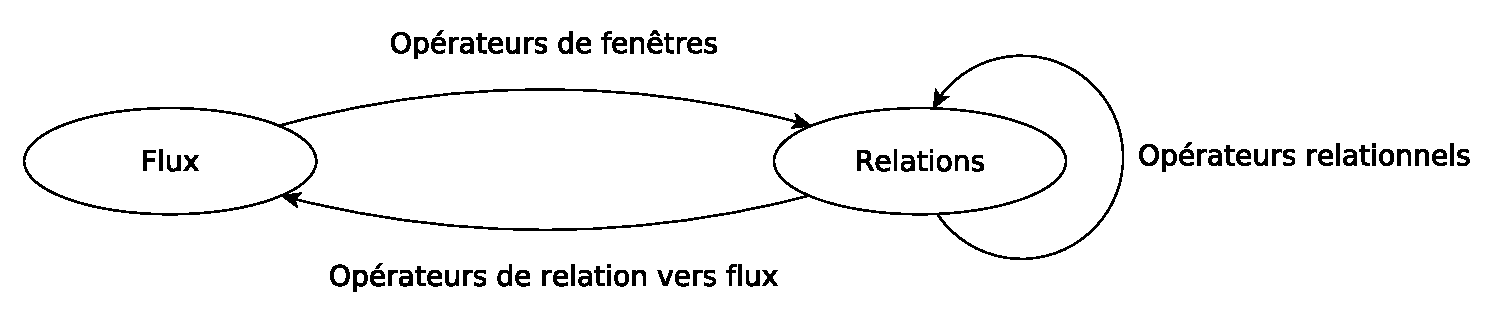
\includegraphics[width=0.75\textwidth]{rw-sgfd-streamrelation}
    \caption{Transformations appliquées dans la sémantique abstraite de STREAM}\label{fig:rw:sgfd:streamrelation}
\end{figure}

Afin de mieux illustrer la sémantique abstraite utilisée, nous allons détailler un exemple plus concret.
\begin{example}
Soit $S$ un flux de capteurs $(\mathrm{temperature}, \textbf{T})$ avec \textbf{T} pour \textit{timestamp} et temperature pour sa mesure. Nous souhaitons faire un agrégat sur 5 min. La composition des opérateurs est la suivante :
\begin{itemize}
\item D'abord un opérateur de fenêtrage $[5min]$ est appliqué. Il transforme le flux en la relation \enquote{\it groupement des 5 dernières minutes} qui évolue au cours du temps.
\item Ensuite un opérateur d'agrégation\footnote{notation simplifiée de l'opérateur d'agrégation sans groupement dont le résultat est une relation avec un seul attribut \textit{avg}} $\mathcal G_{avg(temp)}$ produit une relation avec un seul n-uplet.
\item Enfin, un opérateur de \textup{streaming} est appliqué. Celui-ci peut avoir plusieurs sémantiques. Prenons le plus simple $ISTREAM$ qui permet de créer un flux à partir des insertions dans la relation. Une mise à jour est considérée comme une suppression suivie d'une insertion.
\end{itemize}
La requête finale est : $$ISTREAM(\mathcal G_{avg(temp)}(S[5min]))$$
\end{example}

Le point clé et novateur de cette approche est que les opérateurs de flux vers flux \textbf{n'existent pas}. Ce point est important, car jusqu'à présent tous les opérateurs étaient de cette forme. Par exemple, la jointure de deux flux n'existe pas par essence. Seule la jointure de relations est possible et la création des relations se fait à partir de fenêtres sur des flux. Les auteurs ont justifié cette approche, car l'écriture de requête est plus intuitive et que cela permet de généraliser l'utilisation des vues matérialisées dans le traitement des flux (introduit auparavant dans Chronicle). La spécification de cette sémantique a permis par la suite de décrire le langage associé CQL~\cite{Arasu:cql} (\textit{Continuous Query Language}) dérivé du \textit{SQL} qui est désormais utilisé dans de nombreux produits académiques et commerciaux~\cite{Witkowski:oraclecq,url:sqlstream}.

\begin{example}
La requête \textit{CQL} de l'exemple précédent a la forme suivante : 
\begin{center}
\it ISTREAM(SELECT AVG(temp) as avg FROM S [RANGE 5min])
\end{center}
\end{example}

La sémantique formelle du langage CQL est présentée au complet dans la thèse d'Arvind Arasu~\cite{Arasu:queries}. L'algèbre \textit{ACO} (\textit{Algebra of Continuous Operators}) y est décrite. Les définitions élémentaires sont les suivantes :
\begin{itemize}
 \item[\textbf{Instant} ($\tau$)] : élément de l'ensemble $\mathcal T$, discret et ordonné\footnote{Il est en réalité définit comme un ensemble satisfaisant les axiomes de Peano. En particulier la présence d'un unique successeur. L'instant de départ de l'exécution est le plus petit instant observé $0$.} et représenté par $\N$.
 \item[\textbf{Relation}] : Fonction associant un instant à un multiensemble de n-uplets avec un schéma commun.
 \item[\textbf{Flux}] : Multi-ensemble d'éléments $\left<s,\tau\right>$ où $s$ est un n-uplet respectant un schéma commun et $\tau \in \mathcal T$ son \textit{timestamp}. Pour un $\tau$ donné, il existe un nombre fini (mais non borné) d'éléments.
\end{itemize}
Des opérateurs sont définis sur ces éléments. Les opérateurs relationnels sont simples car pour une \textit{relation} $R$, et un instant $\tau$ : la \textit{relation instantanée} $R(\tau)$ est une relation au sens SGBD\footnote{D'un point de vue strict, les multi-ensembles sont utilisés dans les SGBD mais ne font pas parti du modèle relationnel.}. Les opérateurs classiques peuvent être utilisés. Les équivalences suivantes sont vérifiées : $\forall \tau\in\mathcal T,$ 
\begin{eqnarray*}
    (\sigma_c R)(\tau) & = & \sigma_c(R(\tau))\\
    (R_1 \Join R_2)(\tau) & = & R_1(\tau) \Join R_2(\tau)
\end{eqnarray*}

Les opérateurs les plus importants sont ceux de classe $S2R$ (\textit{stream-to-relation}) et $R2S$ (\textit{relation-to-stream}). La table~\ref{tab:rw:sgfd:acostream} liste les opérateurs présentés.

\begin{table}[ht]
 \centering
\begin{tabular}{|c|c|l|}\bottomrule
Opérateur & Classe & Description \\\toprule \bottomrule
$S[N]$ & $S2R$ & Fenêtre positionnelle glissante de taille $N$ n-uplets \\ \hline
$S[W]_T$ & $S2R$ & Fenêtre temporelle glissante de taille $W$ unités de temps \\\hline
$S[1]_T$ & $S2R$ & Fenêtre représentant l'instant présent\\\hline
$S[\infty]$ & $S2R$ & Fenêtre accumulative\\ \toprule \bottomrule
$\mathcal{IS}(R)$ & $R2S$ & Flux d'insertion \\ \hline
$\mathcal{DS}(R)$ & $R2S$ & Flux de suppression \\ \hline
$\mathcal{RS}(R)$ & $R2S$ & Flux de présence \\ \toprule
\end{tabular}
\caption{Opérateurs de flux de l'algèbre \textit{ACO}}\label{tab:rw:sgfd:acostream}
\end{table}

Pour les \textit{streamers}, leurs définitions sont dérivées de l'état de la relation à l'instant présent ainsi qu'à l'instant précédent. Leurs définitions dépendent de la discrétisation du temps. Soit $R$ une relation,
\begin{eqnarray*}
    \mathcal{IS}(R) & = & \bigcup_{\tau\geq 0} ((R(\tau) - R(\tau-1))\times \{\tau\})\\
    \mathcal{DS}(R) & = & \bigcup_{\tau>0} ((R(\tau-1) - R(\tau))\times \{\tau\})\\
    \mathcal{RS}(R) & = & \bigcup_{\tau\geq 0} (R(\tau)\times \{\tau\})
\end{eqnarray*}
La définition des fenêtres est quant à elle plus technique. L'idée est de regrouper les n-uplets selon un critère particulier. Soit $S$ un flux,
\begin{eqnarray*}
    S[W]_T & = & \left\{s | \left<s,\tau'\right>\in S \wedge (\tau' \leq \tau) \wedge (\tau' \geq \max\{\tau - W +1,0\})   \right\}\\
    S[N] & = & \left\{s_i \in S | \max\{1,n(\tau)-N+1\} \leq i \leq n(\tau)\right\}
\end{eqnarray*}
où la suite $(s_n)$ correspond à la suite des n-uplets ordonnés par \textit{timestamp} et $n(\tau)$ le nombre d'éléments de $S$ possédant un \textit{timestamp} $\leq \tau$.

Le langage \textit{CQL} et l'algèbre \textit{ACO} ont été démontrés comme plus expressifs~\cite{Arasu:cql} que les autres solutions que nous avons mentionnées précédemment (Chronicles, Tribeca, Tapestry, Gigascope, Aurora et TelegraphCQ).

\subsection{Formalisation de la sémantique des opérateurs}\label{sec:rw:sgfd:modeles:batch}
Depuis 2005, plusieurs travaux se sont intéressés à la formalisation de la sémantique des opérateurs. Le plus étudié reste l'opérateur de fenêtrage qui est une des principales raisons de la complexité des systèmes de gestion de flux de données~\cite{Maier:semantics,Patroumpas:window,Patroumpas:subsumewindows}. Une meilleure compréhension de cet opérateur permet de mieux maîtriser la sémantique implantée, mais aussi des optimisations de l'évaluation telles que le partage de résultats (voir section~\ref{sec:rw:sgfd:optim}).

En 2008, les auteurs à l'origine de \textit{STREAM}, d'\textit{Aurora}, de \textit{StreamBase} et d'\textit{OracleCQ} ont présenté~\cite{Jain:spread} pour dénoncer l'ambiguïté sémantique des langages de gestion de flux. En effet, l'exécution des opérateurs complexes tels que les fenêtres n'étaient pas identiques entre l'interprétation de \textit{StreamBase} et l'interprétation d'\textit{Oracle}. Le phénomène s'observe lorsque les modes d'exécutions sont différents.
\begin{itemize}
	\item Le mode basé sur le temps groupe tous les n-uplets qui possèdent le même \textit{timestamp}. Le flux est formé, comme présenté sur la figure~\ref{fig:rw:sgfd:mode:time}, de n-uplets groupés par \textit{timestamp}. Ainsi, les traitements sont exécutés à chaque \textit{timestamp}.
	\begin{figure}[ht]
		\centering
		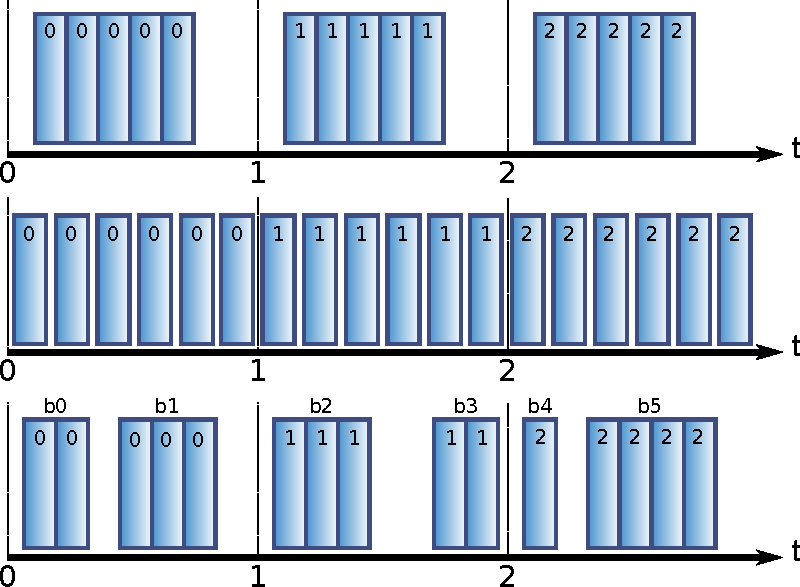
\includegraphics[trim=0mm 66mm 0mm 0mm, clip, width=0.6\textwidth]{rw-sgfd-modes2}
		\caption{Mode d'exécution à base temporelle}\label{fig:rw:sgfd:mode:time}
	\end{figure}
	\item Le mode basé sur les n-uplets au contraire considère que chaque n-uplet est une donnée à part entière. Le \textit{timestamp} n'est qu'une information du n-uplet pouvant être éventuellement utilisé par un opérateur de fenêtre, comme présenté sur la figure~\ref{fig:rw:sgfd:mode:tuple}.
	\begin{figure}[ht]
		\centering
		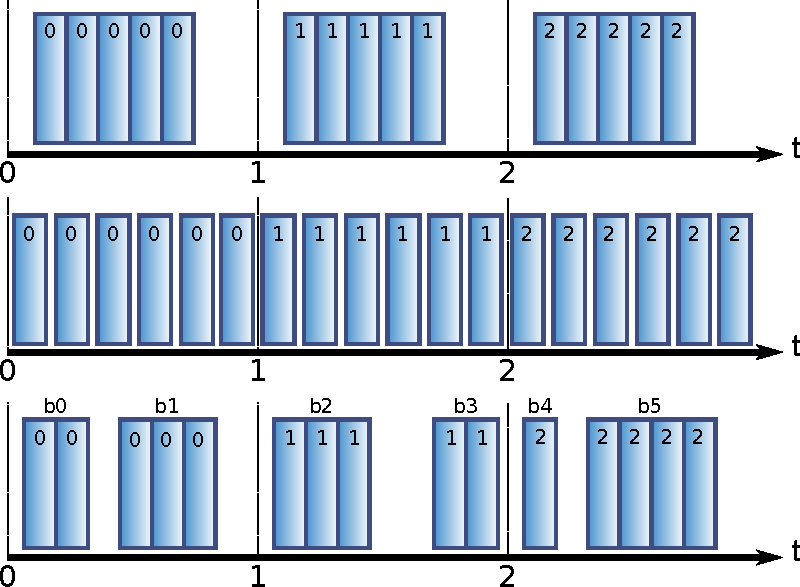
\includegraphics[trim=0mm 33mm 0mm 33mm, clip, width=0.6\textwidth]{rw-sgfd-modes2}
		\caption{Mode d'exécution basé n-uplet}\label{fig:rw:sgfd:mode:tuple}
	\end{figure}
\end{itemize}

Or, ces deux sémantiques rentrent effectivement en conflit sur certaines opérations, en voici un exemple :
\begin{example}\label{ex:rw:sgfd:batches}
 Soit $S$ un flux dont le contenu est, dans le formalisme \textit{ACO}, $\{\left<s_1,0\right>, \left<s_2,0\right>, \left<s_3,1\right>\}$. Nous souhaitons observer le résultat de la requête $S[1]$ (fenêtre de 1-tuple).

Si le modèle d'exécution est basé sur l'arrivée des n-uplets. Alors lorsque le n-uplet $s_1$ entre dans le système. Le système remplit une nouvelle fenêtre, ce qui donne $S[1](0)=\{s_1\}$. 

Le n-uplet $s_2$ est fournit et le système produit une nouvelle fenêtre : $S[1](0)=\{s_2\}$. Cette interprétation permet de considérer tous les n-uplets. Néanmoins, au même instant, la fenêtre a deux états différents, ce qui n'est pas correct d'un point de vue formel.

Si le modèle d'exécution est à base temporelle. Alors à l'instant 0, l'opérateur va obtenir les deux n-uplets. Puis, conformément à sa spécification algébrique, va sélectionner l'un d'eux, pour produire $S[1](0) = \{s_1\}$ ou $\{s_2\}$. Ceci est correct d'un point de vue formel, toutefois cet opérateur va perdre des données, ce qui peut être problématique.
\end{example}

Le problème est que les deux sémantiques ont du sens a priori. Pour clarifier, les auteurs introduisent la notion de \textit{batch}. Le \textit{batch} est une généralisation de ces modes puisqu'il considère que l'ensemble des n-uplets simultanés est partitionné en sous-ensembles ordonnés, comme représentés dans la figure~\ref{fig:rw:sgfd:mode:batch}. Ainsi, l'unité de temps d'exécution n'est pas le \textit{timestamp} ou l'n-uplet, c'est le \textit{batch}.
\begin{figure}[ht]
    \centering
		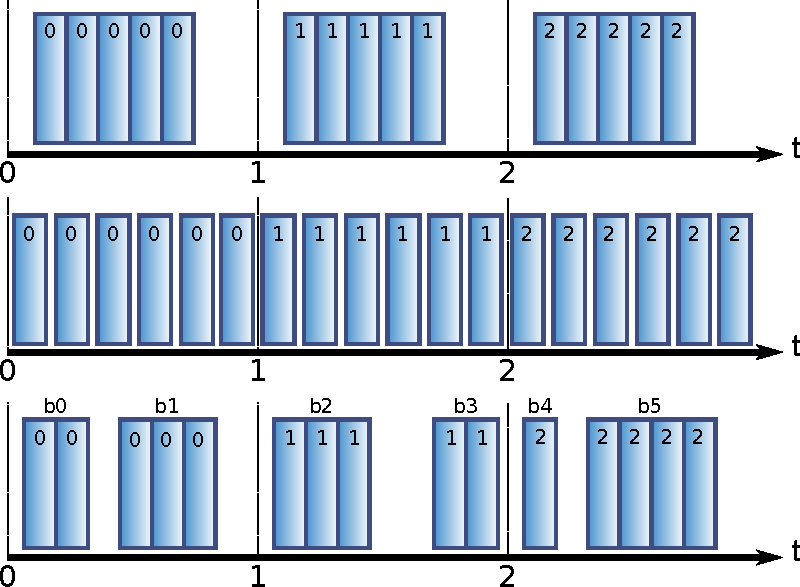
\includegraphics[trim=0mm 0mm 0mm 66mm, clip, width=0.6\textwidth]{rw-sgfd-modes2}
    \caption{Mode d'exécution basé \textit{batch}}\label{fig:rw:sgfd:mode:batch}
\end{figure}

Le \textit{batch} correspond à un envoi groupé de la part de la source. Si deux événements se produisent au même \textit{instant} (à l'unité de temps près)\footnote{Ces cas apparaissent facilement dans les cadres de grande échelle ou lorsqu'un événement est cause d'un autre}, la source effectue quand même deux actions de production de la source, ces productions correspondent à deux \textit{batchs} différents.

Des opérateurs sont développés pour manipuler les \textit{batchs} pour passer d'un mode d'exécution à l'autre. Par exemple, il est possible de structurer les \textit{batchs} d'un \textit{timestamp} donné à partir d'un autre attribut (identifiant par exemple).

De façon similaire, nous pouvons remarquer que dans l'algèbre \textit{ACO} la gestion de l'ordre positionnel est floue. Le flux est ordonné par \textit{timestamp}, mais en cas de n-uplets dits \textit{simultanés}, aucun ordre strict n'est définit. Dans la définition de la fenêtre positionnelle, \textit{ACO} introduit la définition d'une suite $(s_n)$ strictement ordonné. A. Arasu a dit sur ce point dans son manuscrit de thèse~\cite{Arasu:queries} : \enquote{\it Comme nous ordonnons arbitrairement la séquence $s_1$, $s_2$,..., les fenêtres positionnelles sont non déterministes lorsque les \textit{timestamps} ne sont pas uniques, ce qui peut ne pas être approprié}. L'introduction des \textit{batchs} apporte une généralisation de l'ordre temporel, ce qui permet de mieux maîtriser la sémantique d'exécution. Toutefois, s'il est nécessaire de faire un choix d'un nombre limité de n-uplets pour remplir une fenêtre, par exemple, ce choix reste non déterministe.

Suite à l'identification des problèmes de modes d'exécution, le modèle \textit{SECRET}~\cite{Botan:secret} a été développé. Le principe est de décomposer l'opérateur de fenêtre en trois parties. Tout d'abord, le modèle décrit sa portée et son contenu (\textit{scope \& content}) pour savoir quels n-uplets sont inclus dans les fenêtres. Ensuite, les auteurs détaillent son mode de consommation de n-uplet (\textit{tick}), et enfin son mode de notification à l'utilisateur. Cette séparation claire des concepts permet d'avoir une meilleure compréhension des sémantiques possibles sur les fenêtres. Ainsi, ce modèle permet de décrire les modes de fonctionnement de systèmes existants pour mieux permettre leur intégration par la suite.

Les travaux de Krämer~\cite{Kramer:semantics} détaillent une algèbre de manipulation des flux. Le point novateur est la séparation des flux dits\textit{bruts}, \textit{logique} et \textit{physique}. 
\begin{itemize}
	\item Les flux tels que nous les avons décrit dans cette section sont des flux \textit{bruts} composés de couples $(\textrm{n-uplet},\textit{timestamp})$.
	\item Les flux logiques sont quant à eux un ensemble de triplets $(\textrm{n-uplet}, \textit{timestamp}, n)$. La multiplicité $n$ permet de compter le nombre d'occurrences du n-uplet a été observée dans le flux originel.
	\item Les flux physiques utilisent une définition très similaire à ce qui peut se trouver dans les bases de données temporelles avec un intervalle de validité. Ses éléments sont des couples $(\textrm{n-uplet},[t_s, t_e[)$.
\end{itemize} 
Deux algèbres sont ainsi décrites. La première manipule les flux logiques. Elle est utilisable pour correctement comprendre la sémantique des différents opérateurs. La seconde manipule les flux physiques qui sont utilisés par les implémentations des opérateurs. Des équivalences d'expressions sont ensuite définies pour passer du domaine logique au physique.

Enfin, les travaux sur SoCQ~\cite{Gripay:algebra} permettent d'exprimer une algèbre pouvant modéliser des extensions virtuelles aux relations classiques de base de données. Ces extensions apportent des attributs pouvant être issus de flux ou des propriétés virtuelles fournies par des services logiciels\footnote{Au sens architecture à service du terme}. L'avantage d'une telle approche est de pouvoir intégrer rapidement les services issus de l'implémentation avec une gestion des données. Ainsi, nous avons une modélisation des sources mélangeant relations classiques et flux de données.
